% Multi-model pipeline of condition C1 (v2-v3), with C0 and C0g marked. TikZ; compile with pdflatex.
\documentclass[tikz,border=3pt]{standalone}
\usepackage[T1]{fontenc}
\usepackage[scaled=0.92]{helvet}
\renewcommand{\familydefault}{\sfdefault}
\usetikzlibrary{arrows.meta,calc,shapes.geometric,positioning}
\definecolor{wfill}{HTML}{FFFFFF}\definecolor{wline}{HTML}{4D4D4D}
\definecolor{jfill}{HTML}{FBE9D7}\definecolor{jline}{HTML}{D55E00}
\definecolor{gfill}{HTML}{DCEEFB}\definecolor{gline}{HTML}{0072B2}
\definecolor{orfill}{HTML}{E3F4EC}\definecolor{orline}{HTML}{009E73}
\definecolor{outfill}{HTML}{FFF2CC}\definecolor{outline}{HTML}{B07D00}
\definecolor{zone}{HTML}{9A9A9A}
\hyphenpenalty=10000\exhyphenpenalty=10000
\begin{document}
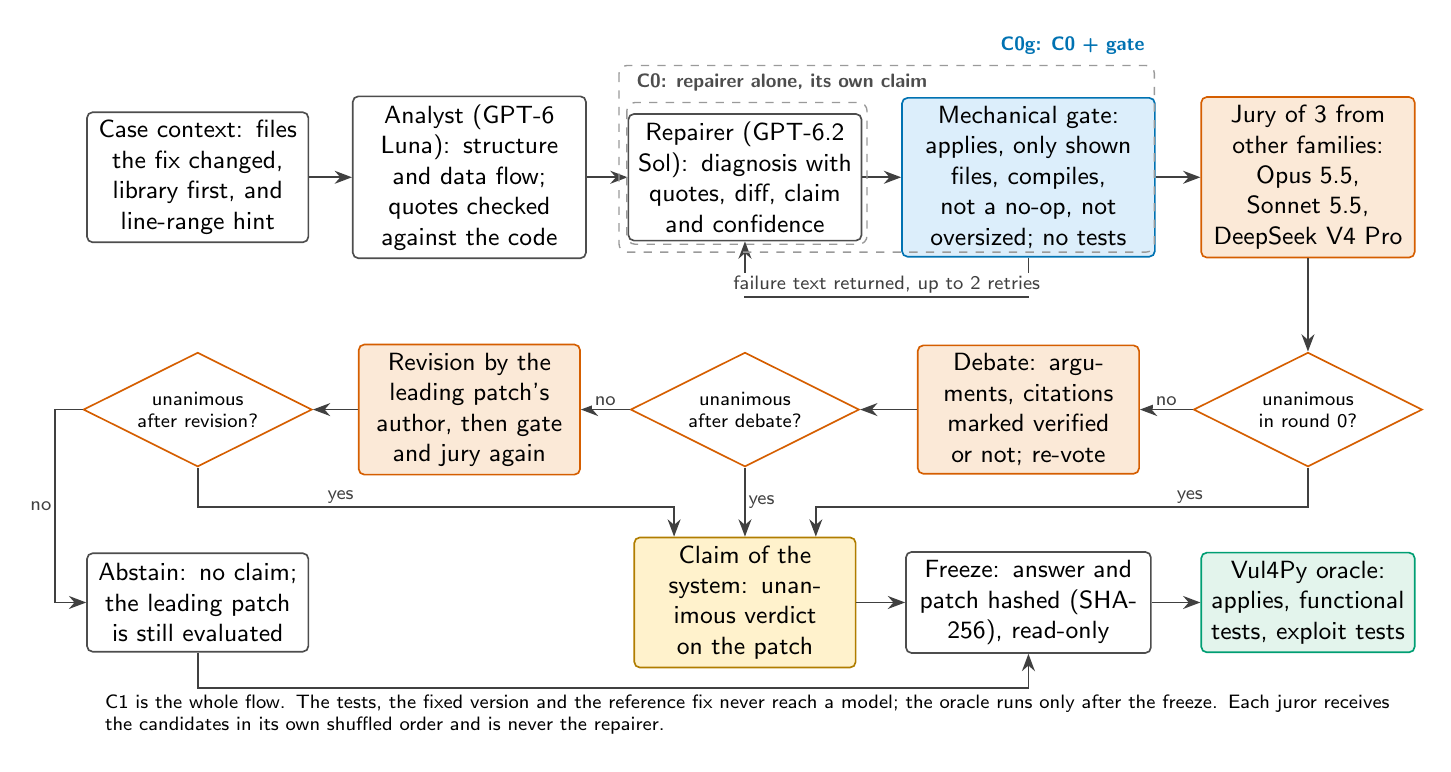
\begin{tikzpicture}[
  font=\small,
  box/.style={draw=wline, fill=wfill, rounded corners=2pt, align=center, text width=#1, minimum height=1.25cm, inner sep=3pt, line width=0.6pt},
  box/.default=2.75cm,
  jury/.style={fill=jfill, draw=jline},
  gate/.style={fill=gfill, draw=gline},
  dec/.style={draw=jline, fill=wfill, diamond, aspect=2.0, align=center, text width=1.9cm, inner sep=0.5pt, line width=0.6pt, font=\scriptsize},
  arr/.style={-{Stealth[length=2.2mm]}, line width=0.6pt, color=black!75},
  lab/.style={font=\scriptsize, fill=white, inner sep=1pt},
  brace/.style={draw=zone, line width=0.5pt, rounded corners=3pt, dashed}
]
% ------------------------------------------------------------ row 1: generation
\node[box=2.6cm] (ctx) at (1.5,0) {Case context: files the fix changed, library first, and line-range hint};
\node[box] (ana) at (4.95,0) {Analyst (GPT-6 Luna): structure and data flow; quotes checked against the code};
\node[box] (rep) at (8.45,0) {Repairer (GPT-6.2 Sol): diagnosis with quotes, diff, claim and confidence};
\node[box=3.0cm, gate] (gt) at (12.05,0) {Mechanical gate: applies, only shown files, compiles, not a no-op, not oversized; no tests};
\node[box=2.5cm, jury] (jur) at (15.6,0) {Jury of 3 from other families: Opus 5.5, Sonnet 5.5, DeepSeek V4 Pro};
% ------------------------------------------------------------ row 2: jury protocol
\node[dec] (u0) at (15.6,-2.95) {unanimous in round 0?};
\node[box=2.6cm, jury] (deb) at (12.05,-2.95) {Debate: arguments, citations marked verified or not; re-vote};
\node[dec] (u1) at (8.45,-2.95) {unanimous after debate?};
\node[box=2.6cm, jury] (rev) at (4.95,-2.95) {Revision by the leading patch's author, then gate and jury again};
\node[dec] (u2) at (1.5,-2.95) {unanimous after revision?};
% ------------------------------------------------------------ row 3: outcome
\node[box=2.6cm, fill=outfill, draw=outline] (claim) at (8.45,-5.4) {Claim of the system: unanimous verdict on the patch};
\node[box=2.6cm] (abst) at (1.5,-5.4) {Abstain: no claim; the leading patch is still evaluated};
\node[box=2.9cm] (frz) at (12.05,-5.4) {Freeze: answer and patch hashed (SHA-256), read-only};
\node[box=2.5cm, fill=orfill, draw=orline] (orc) at (15.6,-5.4) {Vul4Py oracle: applies, functional tests, exploit tests};
% ------------------------------------------------------------ arrows
\draw[arr] (ctx) -- (ana);
\draw[arr] (ana) -- (rep);
\draw[arr] (rep) -- (gt);
\draw[arr] (gt) -- (jur);
\draw[arr] (gt.south) -- ++(0,-0.5) -| node[lab, pos=0.25, above] {failure text returned, up to 2 retries} (rep.south);
\draw[arr] (jur) -- (u0);
\draw[arr] (u0) -- node[lab, above] {no} (deb);
\draw[arr] (deb) -- (u1);
\draw[arr] (u1) -- node[lab, above] {no} (rev);
\draw[arr] (rev) -- (u2);
\draw[arr] (u0.south) -- ++(0,-0.5) -| node[lab, pos=0.12, above] {yes} ($(claim.north)+(0.9,0)$);
\draw[arr] (u1.south) -- node[lab, right] {yes} (claim.north);
\draw[arr] (u2.south) -- ++(0,-0.5) -| node[lab, pos=0.15, above] {yes} ($(claim.north)+(-0.9,0)$);
\draw[arr] (u2.west) -- ++(-0.35,0) |- node[lab, pos=0.25, left] {no} (abst.west);
\draw[arr] (claim) -- (frz);
\draw[arr] (abst.south) -- ++(0,-0.45) -| (frz.south);
\draw[arr] (frz) -- (orc);
% ------------------------------------------------------------ conditions
\draw[brace] (6.95,0.95) rectangle (10.0,-0.85);
\node[font=\scriptsize\bfseries, anchor=south west, text=wline] at (6.95,0.97) {C0: repairer alone, its own claim};
\draw[brace] (6.85,1.42) rectangle (13.65,-0.95);
\node[font=\scriptsize\bfseries, anchor=south east, text=gline] at (13.65,1.44) {C0g: C0 + gate};
\node[font=\scriptsize, anchor=north west, align=left, text width=16.5cm] at (0.2,-6.45)
  {C1 is the whole flow. The tests, the fixed version and the reference fix never reach a model; the oracle runs only after the freeze. Each juror receives the candidates in its own shuffled order and is never the repairer.};
\end{tikzpicture}
\end{document}
